\documentclass
%[handout]
{beamer}
%\documentclass{beamer}

%%
%%
%%
% From http://tex.stackexchange.com/questions/2072/beamer-navigation-circles-without-subsections
% Solution #2 or 3:
% \usepackage{etoolbox}
% \makeatletter
% % replace the subsection number test with a test that always returns true
% \patchcmd{\slideentry}{\ifnum#2>0}{\ifnum2>0}{}{\@error{unable to patch}}%
% \makeatother
% Solution #1:
\usepackage{remreset}% tiny package containing just the \@removefromreset command
\makeatletter
\@removefromreset{subsection}{section}
\makeatother
\setcounter{subsection}{1}


\usepackage{etex}
\usepackage{pgf}
\usepackage{tikz}
\usepackage{url}
\usepackage{amsmath}
\usepackage{color}
% \definecolor{red}{rgb}{1,0,0}
\usepackage{ulem}
% \usepackage{booktabs}
\usepackage{colortbl,booktabs}
\renewcommand*{\thefootnote}{\fnsymbol{footnote}}
\usepackage{fancybox}
\usepackage[framemethod=TikZ]{mdframed}
\mdfdefinestyle{FactStyle}{%
  outerlinewidth=0.5,
  roundcorner=1pt,
  leftmargin=1cm,
  linecolor=blue,
  outerlinecolor=blue!70!black,
  backgroundcolor=yellow!40
}
\usepackage{cancel}

  \newcommand\Warning{%
    \makebox[2.4em][c]{%
      \makebox[0pt][c]{\raisebox{.2em}{\Large!}}%
      \makebox[0pt][c]{\color{red}\Huge$\bigtriangleup$}}}%

\usepackage{stackengine}
\usepackage{scalerel}
\usepackage{xcolor}
  \newcommand\dangersign[1][2ex]{%
    \renewcommand\stacktype{L}%
    \scaleto{\stackon[1.3pt]{\color{red}$\triangle$}{\tiny !}}{#1}%
  }



\usepackage{dcolumn}
\newcolumntype{d}[1]{D{.}{.}{#1}}

% From
% http://tex.stackexchange.com/questions/109900/how-can-i-box-multiple-aligned-equations
\usepackage{empheq}
\usepackage{tcolorbox}  \newtcbox{\othermathbox}[1][]{%
  nobeforeafter, tcbox raise base, 
  colback=black!10, colframe=red!30, 
  left=1em, top=0.5em, right=1em, bottom=0.5em}

\newcommand\blue{\color{blue}}
\newcommand\red{\color{red}}
\newcommand\green{\color{green!75!black}}
\newcommand\purple{\color{purple}}
\newcommand\bluegreen{\color{blue!75!green}}
\newcommand\orange{\color{orange}}
\newcommand\redgreen{\color{red!50!green}}
\newcommand\grey{\color{black}}
\newcommand\gap{\vspace{.1in}}
\newcommand\nb{${\red\bullet}\ $}
\newcommand\halfgap{\vspace{.05in}}
\newcommand\divideline{\line(1,0){352}}
\usepackage{marvosym} % for \Smiley

\newcommand{\bluealert}[1]{{\blue\textbf{#1}}}

% \usepackage{beamerthemesplit} %Key package for beamer
\usetheme{Singapore}
% \usetheme{Szeged}
% \usetheme{Garfield}
% \usetheme{CambridgeUS}
% \usenavigationsymbolstemplate{} %Gets rid of slide navigation symbols


\setbeamercolor{separation line}{use=structure,bg=structure.fg!50!bg}
% \begin{beamercolorbox}[colsep=0.5pt]
%   {upper separation line foot}
% \end{beamercolorbox}



\makeatletter
\setbeamertemplate{footline}
{
  \leavevmode%
  \hbox{%
% \begin{beamercolorbox}[colsep=0.5pt]
%   {upper separation line foot}
% \end{beamercolorbox}


  \begin{beamercolorbox}[wd=.5\paperwidth,ht=2.25ex,dp=2ex,colsep=0.5pt]%
    {upper separation line foot}
    \usebeamerfont{author in head/foot}%
    \hspace*{2ex}\insertshortdate:\ \insertshorttitle
  \end{beamercolorbox}%
  \begin{beamercolorbox}[wd=.5\paperwidth,ht=2.25ex,dp=2ex,right]{title in head/foot}%
    \usebeamerfont{title in head/foot}
    {\insertshortauthor}\hspace*{2ex}
  \end{beamercolorbox}}%
  % \begin{beamercolorbox}[wd=.333333\paperwidth,ht=2.25ex,dp=2ex,right]{date in head/foot}%
  %   \usebeamerfont{date in head/foot}\insertshortdate{}\hspace*{2em}
  %   \insertframenumber{} / \inserttotalframenumber\hspace*{2ex} 
  % \end{beamercolorbox}%
  \vskip0pt%
}
\makeatother

\usetikzlibrary{decorations.markings}
\usetikzlibrary{arrows}


\title{Final Exam Review}
\author{Peter Garfield, UCSB Mathematics}
\date{March 15, 2017}
%\institute{}


\useinnertheme{default}

\usefonttheme{serif}
% \usecolortheme{rose}
% \usecolortheme{whale}
% \usecolortheme{orchid}
\usecolortheme{crane}
% \usecolortheme{dolphin}


%TEMPLATE
\setbeamertemplate{navigation symbols}{}

\setbeamertemplate{note page}[compress]

\setbeamertemplate{frametitle}{
  \vspace{0.5em}
  % \begin{centering}
  {\huge\blue\textbf{\textmd{\insertframetitle}}}
  \par
  % \end{centering}
}

% From http://tex.stackexchange.com/questions/7032/good-way-to-make-textcircled-numbers:
\newcommand*\circled[1]{\tikz[baseline=(char.base)]{\node[shape=circle,draw,fill=orange,inner sep=1pt] (char) {#1};}} 
% \renewcommand{\labelenumi}{\circled{\textbf{\arabic{enumi}}}}

\let\olddescription\description
\let\oldenddescription\enddescription
\usepackage{enumitem}
\let\description\olddescription
\let\enddescription\oldenddescription

% \usepackage[loadonly]{enumitem}
\setlist[enumerate,1]{label=\colorbox{orange}{\arabic*.},font=\bfseries}
%\setlist[enumerate,2]{label=\colorbox{blue!25}{(\alph*)},font=\bfseries}
% \setlist[enumerate,1]{label=\arabic*.,font=\bfseries}
\setlist[itemize,1]{label=\red$\bullet$}
\setlist[itemize,2]{label=\blue$\bullet$}

\newcommand\answer[1]{\fbox{#1}}
% \renewcommand\answer[1]{}

\newcommand{\antilog}{\operatorname{antilog}}







\title{}
\title{Lines}
\date{April 7, 2022}


\begin{document}
\section{Introduction}
\frame{
  \frametitle{}
  {\Huge{}Welcome To Math 34A!}\\[.5em]

  {\Huge{}Differential Calculus}
  \vfill
  {\Large{}Instructor:}\\
  \ \hspace*{0.2in} Nathan Schley ({\it Sh}+{\it lye}), \url{schley@math.ucsb.edu}\\
  \ \hspace*{0.2in} South Hall 6701
  \\[0.5em]

  {\Large{}Office Hours:}\\
  \ \hspace*{0.2in} T R 11-11:50, T 3:45-4:35 Details on Gauchospace. 
  \bigskip

  \copyright\ 2017-22\ Daryl Cooper, Peter M.\ Garfield, Ebrahim Ebrahim \& Nathan Schley\\
  Please do not distribute outside of this course.
  \vfill

}

\frame{
  \frametitle{Warm-up}

  {\large \blue How many times do we need to double 1 to get the following numbers? }
  \pause   
  \begin{itemize} 
  \item 4 \pause \ \ \fbox{2}
  \pause
  \item 8 \pause \ \ \fbox{3}
  \pause
  \item 32 \pause \  \fbox{5}
  \pause
  \item 1 \pause \ \ \fbox{0}
  \pause
  \item $\frac{1}{2}$ \pause \ \ \fbox{-1}
  
  \end{itemize}
  
  
  

} 

\section*{Slope of a Line}

\frame{
  \frametitle{Straight Lines (\S 6.1)}

  Calculus is about {\red{}derivatives (Math 34A)}\ and
  {\blue{}integrals (Math 34B)}.
  \pause
  \halfgap

  A {\red{}derivative}\ is the slope of a line.
  \pause = {\blue RISE}/{\red RUN}

  \begin{center}
    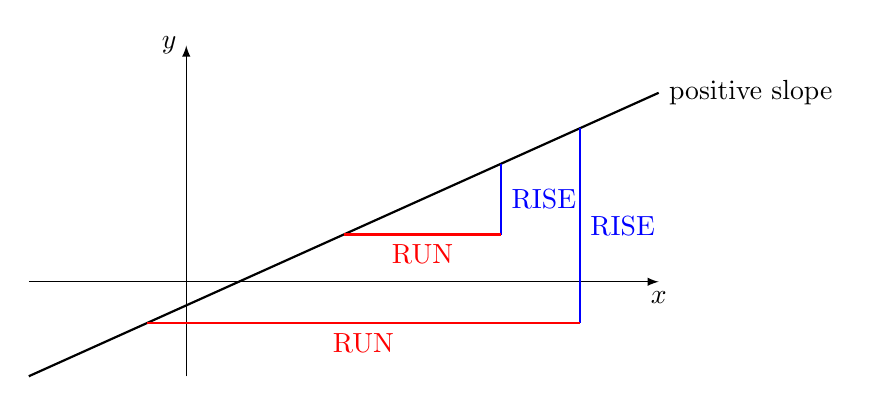
\begin{tikzpicture}[x=10mm,y=6mm,>=latex]
      \draw[thin,black,->] (-2,0) -- (6,0) node[below] {$x$};
      \draw[thin,black,->] (0,-2) -- (0,5) node[left] {$y$};
      % y=-2+(3/4)*(x+2) or y=3/4 x - 1/2 = (3x-2)/4
      \draw[thick,black] (-2,-2) -- (6,4) node[right] {positive slope};
      \draw[thick,blue] (4,{(3*2-2)/4}) -- (4,{(3*4-2)/4}) node[midway,right] {RISE};
      \draw[thick,red] (2,{(3*2-2)/4}) -- (4,{(3*2-2)/4}) node[midway,below] {RUN};
      \uncover<4->{%
        \draw[thick,blue] (5,{(3*-0.5-2)/4}) -- (5,{(3*5-2)/4}) node[midway,right] {RISE};
        \draw[thick,red] (-0.5,{(3*-0.5-2)/4}) -- (5,{(3*-0.5-2)/4}) node[midway,below] {RUN};
      }
    \end{tikzpicture}
  \end{center}

} 

\frame{
  \frametitle{Examples}

  \begin{enumerate}
    \setcounter{enumi}{0}
  \item  What is the slope here?
    \vspace*{-1em}
  \begin{center}
    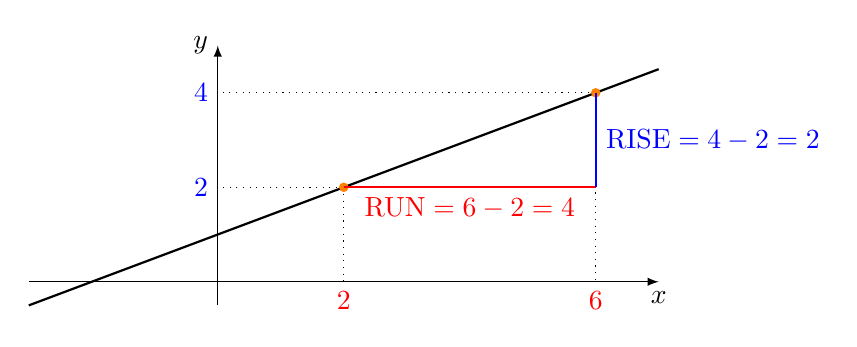
\begin{tikzpicture}[x=8mm,y=6mm,>=latex]
      \draw[thin,black,->] (-3,0) -- (7,0) node[below] {$x$};
      \draw[thin,black,->] (0,-0.5) -- (0,5) node[left] {$y$};
      % y=-2+(3/4)*(x+2) or y=3/4 x - 1/2 = (3x-2)/4
      % m=5/10 = 1/2, so y=4+(1/2)*(x-6) or y=x/2+1:
      \draw[thick,black] (-3,-0.5) -- (7,4.5);
      % \draw[thick,blue] (4,{(3*2-2)/4}) -- (4,{(3*4-2)/4}) node[midway,right] {RISE};
      % \draw[thick,red] (2,{(3*2-2)/4}) -- (4,{(3*2-2)/4}) node[midway,below] {RUN};
      % \uncover<4->{%
      %   \draw[thick,blue] (5,{(3*-0.5-2)/4}) -- (5,{(3*5-2)/4}) node[midway,right] {RISE};
      %   \draw[thick,red] (-0.5,{(3*-0.5-2)/4}) -- (5,{(3*-0.5-2)/4}) node[midway,below] {RUN};
      % }
      \draw[thin,black,dotted] (2,2) -- (2,0) node[below,red] {$2$};
      \draw[thin,black,dotted] (2,2) -- (0,2) node[left,blue] {$2$};
      \draw[thin,black,dotted] (6,4) -- (6,0) node[below,red] {$6$};
      \draw[thin,black,dotted] (6,4) -- (0,4) node[left,blue] {$4$};
      \filldraw[orange] (2,2) circle (1.5pt);
      \filldraw[orange] (6,4) circle (1.5pt);
      \uncover<2->{%
        \draw[thick,red] (2,2) -- (6,2) node[midway,below]{$\text{RUN}=6-2=4$};
        \draw[thick,blue] (6,2) -- (6,4) node[midway,right]{$\text{RISE}=4-2=2$};
      }
    \end{tikzpicture}
  \end{center}
  \end{enumerate}
  \vspace*{-1.5em}

  \begin{center}
    A$=3$
    \qquad
    B$=3/2$
    \qquad
    C$=1$
    \qquad
    D$=1/2$
    \qquad
    E$=\text{other}$
    \qquad
    \uncover<2->{\fbox{D}}
  \end{center}
  \pause

  slope = \#\ units {\blue UPWARDS}\ you move for each unit you move\ {\red{}TO THE RIGHT}
  \pause

  Idea: \parbox[t]{3.75in}{%
      $\text{{\blue RISE}}=\text{{\orange slope}}\times\text{{\red RUN}}$\pause
      \qquad
      So if $\text{{\red RUN}}={\red 1}$ then {\blue RISE}={\orange slope}.
    }
    \halfgap
    \pause
 
  A 10\% gradient on a mountain road is a {\orange slope} of $1/10$. 
  It means for every 10 feet you move horizontally you go up (or down) 1 foot.

}

\frame{
  \frametitle{Examples (page 2)}

  \begin{enumerate}
    \setcounter{enumi}{1}
  \item  What is the slope here:
    \begin{center}
      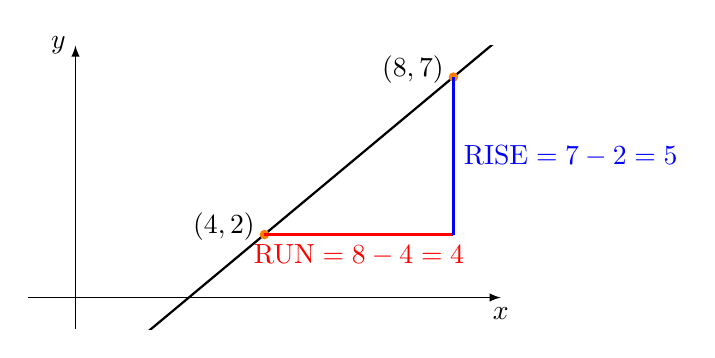
\begin{tikzpicture}[x=6mm,y=4mm,>=latex]
        \draw[thin,black,->] (-1,0) -- (9,0) node[below] {$x$};
        \draw[thin,black,->] (0,-1) -- (0,8) node[left] {$y$};
        \begin{scope}
          \clip (-1,-1) rectangle (9,8);
          % line thru (4,2) and (8,7):
          \draw[thick,black] plot[domain=-1:9] (\x,{2+5*(\x-4)/4});
        \end{scope}
        % y=-2+(3/4)*(x+2) or y=3/4 x - 1/2 = (3x-2)/4
        % m=5/10 = 1/2, so y=4+(1/2)*(x-6) or y=x/2+1:
        % \draw[thick,black] (-3,-0.5) -- (7,4.5);
        % \draw[thick,blue] (4,{(3*2-2)/4}) -- (4,{(3*4-2)/4}) node[midway,right] {RISE};
        % \draw[thick,red] (2,{(3*2-2)/4}) -- (4,{(3*2-2)/4}) node[midway,below] {RUN};
        % \uncover<4->{%
        % \draw[thick,blue] (5,{(3*-0.5-2)/4}) -- (5,{(3*5-2)/4}) node[midway,right] {RISE};
        % \draw[thick,red] (-0.5,{(3*-0.5-2)/4}) -- (5,{(3*-0.5-2)/4}) node[midway,below] {RUN};
        % }
        %   \draw[thin,black,dotted] (2,2) -- (2,0) node[below,red] {$2$};
        %   \draw[thin,black,dotted] (2,2) -- (0,2) node[left,blue] {$2$};
        %   \draw[thin,black,dotted] (6,4) -- (6,0) node[below,red] {$6$};
        %   \draw[thin,black,dotted] (6,4) -- (0,4) node[left,blue] {$4$};
        \filldraw[orange] (4,2) circle (1.5pt) node[black,left,yshift=1mm] {$(4,2)$};
        \filldraw[orange] (8,7) circle (1.5pt) node[black,left,yshift=1mm] {$(8,7)$};
        \uncover<2->{%
          \draw[thick,red] (4,2) -- (8,2) node[midway,below]{$\text{RUN}=8-4=4$};
          \draw[thick,blue] (8,2) -- (8,7) node[midway,right]{$\text{RISE}=7-2=5$};
        }
      \end{tikzpicture}
    \end{center}
    \begin{center}
      A$=5/4$
      \quad 
      B$ = 4/5$
      \quad 
      C$ =1/4$
      \quad
      D$ =4$
      \quad 
      E$ =5$
      \qquad
      \uncover<3->{\fbox{A}}
    \end{center}
  \end{enumerate}

}

\frame{
  \frametitle{Examples (page 3)}

  \begin{enumerate}
    \setcounter{enumi}{2}
  \item  What is the slope here:
    \begin{center}
      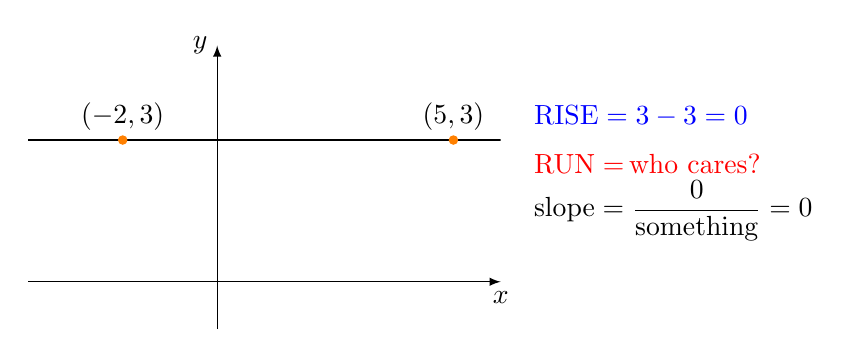
\begin{tikzpicture}[x=6mm,y=6mm,>=latex]
        \draw[thin,black,->] (-4,0) -- (6,0) node[below] {$x$};
        \draw[thin,black,->] (0,-1) -- (0,5) node[left] {$y$};
        \begin{scope}
          \clip (-4,-1) rectangle (6,5);
          % line thru (4,2) and (8,7):
          \draw[thick,black] plot[domain=-4:6] (\x,3);
        \end{scope}
        \filldraw[orange] (-2,3) circle (1.5pt) node[black,above] {$(-2,3)$};
        \filldraw[orange] (5,3) circle (1.5pt) node[black,above] {$(5,3)$};
        \uncover<2->{%
          \node[blue,right] at (6.5,3.5) {$\text{RISE}=3-3=0$};
        }
        \uncover<3->{%
          \node[red,right] at (6.5,2.5) {$\text{RUN}=$\,who cares?};
        }
        \uncover<4->{%
          \node[right] at (6.5,1.5) {$\displaystyle\text{slope}=\frac{0}{\text{something}}=0$};
        }
      \end{tikzpicture}
    \end{center}
    \begin{center}
      A$=0$
      \quad 
      B$ = 7$
      \quad 
      C$ =5/3$
      \quad
      D$ =\infty$
      \quad 
      E$ =3/5$
      \qquad
      \uncover<4->{\fbox{A}}
    \end{center}
  \end{enumerate}

}


\frame{
  \frametitle{Examples (big finish!)}

  \begin{enumerate}
    \setcounter{enumi}{3}
  \item  What is the slope here:
    \begin{center}
      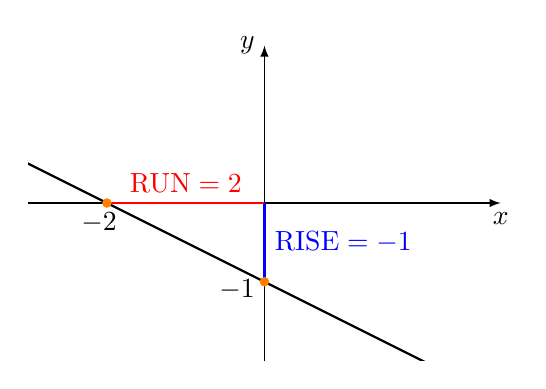
\begin{tikzpicture}[x=10mm,y=10mm,>=latex]
        \draw[thin,black,->] (-3,0) -- (3,0) node[below] {$x$};
        \draw[thin,black,->] (0,-2) -- (0,2) node[left] {$y$};
        \begin{scope}
          \clip (-3,-2) rectangle (3,2);
          % line thru (-2,0) and (0,-1):
          \draw[thick,black] plot[domain=-4:6] (\x,{-1*\x/2-1});
        \end{scope}
        % \foreach \x in {-2} 
        % {
        %   \draw[thin,black] (\x,0) -- (\x,-3mm) node[below] {$\x$};
        % }
        % \foreach \y in {-1} 
        % {
        %   \draw[thin,black] (0,\y) -- (-3mm,\y) node[left] {$\y$};
        % }
        \uncover<2->{%
          \draw[thick,blue] (0,0) -- (0,-1) node[midway,right] {$\text{RISE}=-1$};
          \draw[thick,red] (0,0) -- (-2,0) node[midway,above] {$\text{RUN}=2$};
          % \draw[thick,blue] (0,0) -- (0,-1) node[midway,right] {$\text{RISE}=-1-0=-1$};
          % \draw[thick,red] (0,0) -- (-2,0) node[midway,above] {$\text{RUN}=0-(-2)=2$};
        }
        \filldraw[orange] (-2,0) circle (1.5pt) node[black,below,xshift=-1mm] {$-2$};
        \filldraw[orange] (0,-1) circle (1.5pt) node[black,left,yshift=-1mm] {$-1$};
      \end{tikzpicture}
    \end{center}
    \begin{center}
      A$=-1$
      \quad 
      B$ = 1$
      \quad 
      C$ =1/2$
      \quad
      D$ =-1/2$
      \quad 
      E$ =-2$
      \qquad
      \uncover<3->{\fbox{D}}
    \end{center}
  \end{enumerate}

}


\frame{ 
  \frametitle{General Case}

  \begin{enumerate}
    \setcounter{enumi}{4}
  \item 
    A line goes through two points: $(x_0,y_0)$ and $(x_1,y_1)$.  Find
    the slope of this line.  \alert{\emph{Draw a picture!}}

    \begin{center}
      A$ = y_1-y_0$
      \quad 
      B$=(y_1-x_1)/(y_0-x_0)$
      \quad 
      C$=(y_1-y_0)(x_1-x_0)$
      \medskip

      D$=(y_1-y_0)/(x_1-x_0)$
      \quad 
      E$ = \text{Shirley you're joking}$
      \quad
      \uncover<4->{\fbox{D}}
    \end{center}
  \end{enumerate}
  \halfgap

  \uncover<2->{%
    \begin{center}
      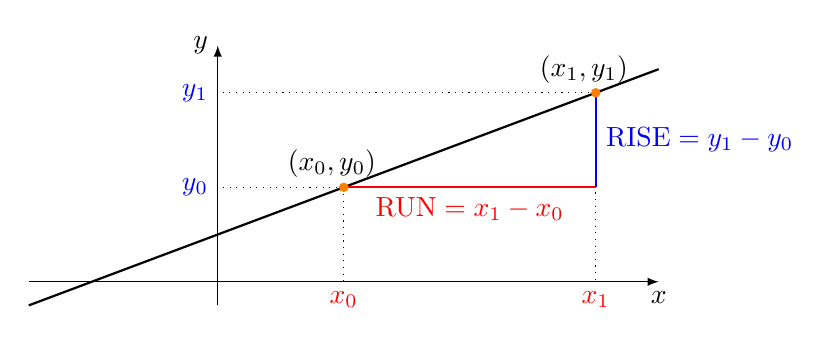
\begin{tikzpicture}[x=8mm,y=6mm,>=latex]
        \draw[thin,black,->] (-3,0) -- (7,0) node[below] {$x$};
        \draw[thin,black,->] (0,-0.5) -- (0,5) node[left] {$y$};
        % y=-2+(3/4)*(x+2) or y=3/4 x - 1/2 = (3x-2)/4
        % m=5/10 = 1/2, so y=4+(1/2)*(x-6) or y=x/2+1:
        \draw[thick,black] (-3,-0.5) -- (7,4.5);
        % \draw[thick,blue] (4,{(3*2-2)/4}) -- (4,{(3*4-2)/4}) node[midway,right] {RISE};
        % \draw[thick,red] (2,{(3*2-2)/4}) -- (4,{(3*2-2)/4}) node[midway,below] {RUN};
        % \uncover<4->{%
        % \draw[thick,blue] (5,{(3*-0.5-2)/4}) -- (5,{(3*5-2)/4}) node[midway,right] {RISE};
        % \draw[thick,red] (-0.5,{(3*-0.5-2)/4}) -- (5,{(3*-0.5-2)/4}) node[midway,below] {RUN};
        % }
        \draw[thin,black,dotted] (2,2) -- (2,0) node[below,red] {$x_0$};
        \draw[thin,black,dotted] (2,2) -- (0,2) node[left,blue] {$y_0$};
        \draw[thin,black,dotted] (6,4) -- (6,0) node[below,red] {$x_1$};
        \draw[thin,black,dotted] (6,4) -- (0,4) node[left,blue] {$y_1$};
        \uncover<3->{%
          \draw[thick,red] (2,2) -- (6,2) node[midway,below]{$\text{RUN}=x_1-x_0$};
          \draw[thick,blue] (6,2) -- (6,4) node[midway,right]{$\text{RISE}=y_1-y_0$};
        }
        \filldraw[orange] (2,2) circle (1.5pt) node[black,above,xshift=-1.5mm] {$(x_0,y_0)$};
        \filldraw[orange] (6,4) circle (1.5pt) node[black,above,xshift=-1.5mm] {$(x_1,y_1)$};
      \end{tikzpicture}
    \end{center}
  }
  \uncover<4->{%
    \begin{equation*}
      \text{Slope} 
      = \frac{\text{\blue{}RISE}}{\text{\red{}RUN}}
      = \frac{{\blue y_1- y_0}}{{\red x_1- x_0}}
    \end{equation*}
  }
} 


\section*{Equation of a Line}


\frame{ 
  \frametitle{The Equation of a Line}

  \alert{The Slope Intercept Form}\ 

  The \textbf{slope intercept}\ equation of a straight line is \ \fbox{$y = {\color{blue}m}x + {\color{red}b}$}\,.

  \begin{center}
    \begin{tikzpicture}[x=8mm,y=6mm,>=latex]
      \draw[thin,black,->] (-3,0) -- (7,0) node[below] {$x$};
      \draw[thin,black,->] (0,-0.5) -- (0,5) node[left] {$y$};
      % y=-2+(3/4)*(x+2) or y=3/4 x - 1/2 = (3x-2)/4
      % m=5/10 = 1/2, so y=4+(1/2)*(x-6) or y=x/2+1:
      \draw[thick,black] (-3,-0.5) -- (7,4.5) node[right] {$y=mx+b$};
      \filldraw[red] (0,1) circle (1.5pt) node[red,left,yshift=1.5mm] {$b$};
    \end{tikzpicture}
  \end{center}
  \vspace*{-1.5em}

  \begin{align*}
    {\color{blue}m} & = \text{the \textbf{slope}.  CRUCIAL for calculus.} \\
    {\color{red}b}  & =\, \text{where the line crosses\ the $y$-axis (the ``$y$-intercept'').}
  \end{align*}
  \pause  
  WHY? Because when you plug in $x=0$, you get $y={\color{red}b}$.

}

\frame{
  \frametitle{Example}

  \begin{enumerate}
    \setcounter{enumi}{5}
  \item Find the equation of the line \fbox{$y={\blue m}x+{\red b}$}
    through the points $(1,3)$ and $(7,5)$.
  \bigskip

  Plan: Find $m$, then find $b$.
  \bigskip

  \begin{itemize}
  \item 
    What is $m$?
    \begin{center}
      A$=1$
      \quad 
      B$=3$
      \quad 
      C$=5$
      \quad 
      D$=1/3$
      \quad 
      E$=2$
      \quad
      \pause
      \fbox{D}
    \end{center}
    \bigskip
    \pause

    So $\displaystyle{}y=\frac{1}{3}x + b$.  What is $b$?  Plug in
    either point!
    \bigskip

    \item What do you get for ${\red b}$?
      \begin{center}
        A$=1/3$
        \quad 
        B$= 4/3$
        \quad 
        C$= 7/3$
        \quad 
        D$= 8/3$
        \quad
        E$= 10/3$ 
        \pause
        \quad
        \fbox{D}
      \end{center}

      \halfgap

      Can we check?
      \pause
    \end{itemize}
  \end{enumerate}

}

\frame{
  \frametitle{You Try It}

  \begin{enumerate}
    \setcounter{enumi}{6}
  \item  A line has slope $1/2$ and goes through the point $(2,5).$
    What is the $y$-coordinate of the point on this line where $x=6$?
    \bigskip
    \begin{center}
      A$=3$
      \qquad 
      B$=4$
      \qquad 
      C$=5$
      \qquad 
      D$=6$
      \qquad 
      E$=7$ 
      \quad
      \uncover<3->{\fbox{E}}
    \end{center}
    \pause
    \bigskip

    \uncover<2->{%
      \alert{Plan:}\ 
      \parbox[t]{2in}{%
        1.\ Find equation of the line. \\
        2.\ Plug in $x=6$ to find $y$.
      }
    }
  \end{enumerate}
  \vspace*{1in}
  \ 
}


\frame{
  \frametitle{Another Equation of a Line}

  \alert{The Point-Slope Form}\ 

  The \textbf{point slope}\ equation of a straight line is \ \fbox{$y = {\color{red}y_0}+{\color{blue}m}(x - {\color{red}x_0})$}\,.

  \begin{center}
    \begin{tikzpicture}[x=8mm,y=6mm,>=latex]
      \draw[thin,black,->] (-3,0) -- (7,0) node[below] {$x$};
      \draw[thin,black,->] (0,-0.5) -- (0,5) node[left] {$y$};
      % y=-2+(3/4)*(x+2) or y=3/4 x - 1/2 = (3x-2)/4
      % m=5/10 = 1/2, so y=4+(1/2)*(x-6) or y=x/2+1:
      \draw[thick,black] (-3,-0.5) -- (7,4.5);% node[right] {$y=mx+b$};
      \filldraw[red] (2,2) circle (1.5pt) node[red,above,xshift=-2.5mm] {\small$(x_0,y_0)$};
      \draw[red,thin,dotted] (2,2) -- (2,0) node[below] {$x_0$};
      \draw[red,thin,dotted] (2,2) -- (0,2) node[left] {$y_0$};
    \end{tikzpicture}
  \end{center}
  \vspace*{-1.5em}

  \begin{align*}
    {\color{blue}m} & = \text{the \textbf{slope}.  Still CRUCIAL for calculus.} \\
    {\color{red}(x_0,y_0)}  & =\, \text{any point on the line.}
  \end{align*}

}

\frame{
  \frametitle{Why Does This Work?}

  \begin{center}
    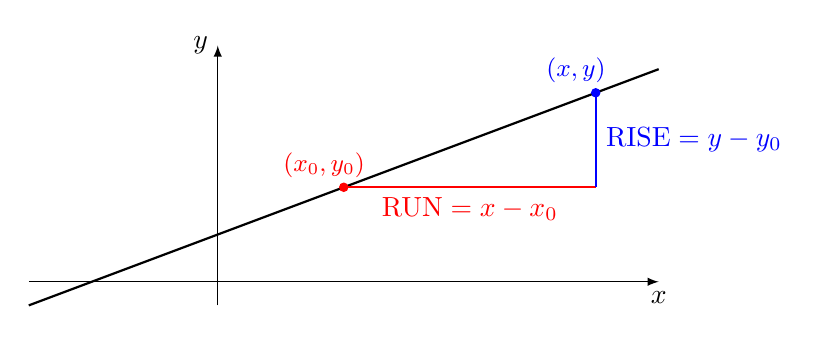
\begin{tikzpicture}[x=8mm,y=6mm,>=latex]
      \draw[thin,black,->] (-3,0) -- (7,0) node[below] {$x$};
      \draw[thin,black,->] (0,-0.5) -- (0,5) node[left] {$y$};
      % y=-2+(3/4)*(x+2) or y=3/4 x - 1/2 = (3x-2)/4
      % m=5/10 = 1/2, so y=4+(1/2)*(x-6) or y=x/2+1:
      \draw[thick,black] (-3,-0.5) -- (7,4.5);
      \filldraw[red] (2,2) circle (1.5pt) node[red,above,xshift=-2.5mm] {\small$(x_0,y_0)$};
      \uncover<2->{%
        \filldraw[blue] (6,4) circle (1.5pt) node[above,xshift=-2.5mm] {\small$(x,y)$};
        \draw[thick,red] (2,2) -- (6,2) node[midway,below]{$\text{RUN}=x-x_0$};
        \draw[thick,blue] (6,2) -- (6,4) node[midway,right]{$\text{RISE}=y-y_0$};
      }
      % \draw[red,thin,dotted] (2,2) -- (2,0) node[below] {$x_0$};
      % \draw[red,thin,dotted] (2,2) -- (0,2) node[left] {$y_0$};
    \end{tikzpicture}
  \end{center}
  \vspace*{-1.5em}

  \begin{align*}
    \text{$(x,y)$ lies on the line}
    & \ \text{exactly when} 
    && \uncover<3->{\frac{y-y_0}{x-x_0} = m} \\
    &&& \uncover<4->{y-y_0 = m(x-x_0)} \\
    &&& \uncover<5->{y=y_0 + m(x-x_0)}
  \end{align*}

}

\frame{
  \frametitle{Examples}

  \begin{enumerate}
    \setcounter{enumi}{7}
  \item Find the equations of these lines (whose slopes we've already
    found):
  \end{enumerate}

  \begin{center}
    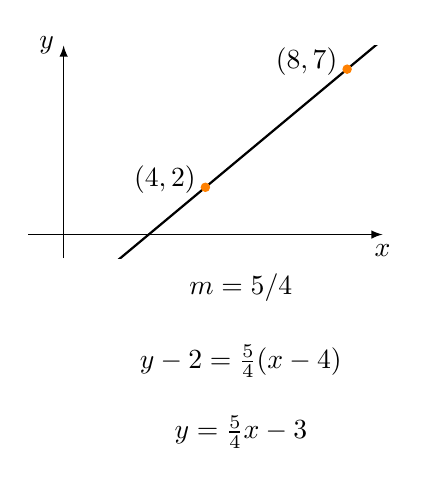
\begin{tikzpicture}[x=4.5mm,y=3mm,>=latex]
      \draw[thin,black,->] (-1,0) -- (9,0) node[below] {$x$};
      \draw[thin,black,->] (0,-1) -- (0,8) node[left] {$y$};
      \begin{scope}
        \clip (-1,-1) rectangle (9,8);
        % line thru (4,2) and (8,7):
        \draw[thick,black] plot[domain=-1:9] (\x,{2+5*(\x-4)/4});
      \end{scope}
      \filldraw[orange] (4,2) circle (1.5pt) node[black,left,yshift=1mm] {$(4,2)$};
      \filldraw[orange] (8,7) circle (1.5pt) node[black,left,yshift=1mm] {$(8,7)$};
      \node[below] at (5,-1.25) {$m=5/4$};
      \uncover<2->{%
        \node[below] at (5,-4.25) {$y-2=\frac{5}{4}(x-4)$};
      }
      \uncover<3->{%
        \node[below] at (5,-7.25) {$y=\frac{5}{4}x-3$};
      }
    \end{tikzpicture}
    \hspace*{6mm}
    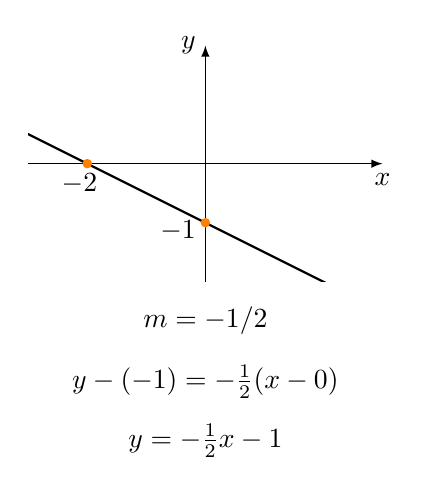
\begin{tikzpicture}[x=7.5mm,y=7.5mm,>=latex]
      \draw[thin,black,->] (-3,0) -- (3,0) node[below] {$x$};
      \draw[thin,black,->] (0,-2) -- (0,2) node[left] {$y$};
      \begin{scope}
        \clip (-3,-2) rectangle (3,2);
        % line thru (-2,0) and (0,-1):
        \draw[thick,black] plot[domain=-4:6] (\x,{-1*\x/2-1});
      \end{scope}
      \filldraw[orange] (-2,0) circle (1.5pt) node[black,below,xshift=-1mm] {$-2$};
      \filldraw[orange] (0,-1) circle (1.5pt) node[black,left,yshift=-1mm] {$-1$};
      \node[below] at (0,-2.25) {$m=-1/2$};
      \uncover<4->{%
        \node[below] at (0,-3.25) {$y-(-1)=-\frac{1}{2}(x-0)$};
      }
      \uncover<5->{%
        \node[below] at (0,-4.25) {$y=-\frac{1}{2}x-1$};
      }
    \end{tikzpicture}
  \end{center}


}


\frame{
  \frametitle{And\ldots?}

  Yes, but what's this got to do with calculus?\\ \pause
  {\red Derivatives} are about \textbf{\color{blue}rate of change}
  and that is what {\blue\textbf{slope}}\ is!\\ \pause
  \gap

  \alert{Example:}\ This graph shows the temperature in an oven as it heats up:
  \begin{center}
    % \includegraphics[scale=0.7]{lines7small} 
    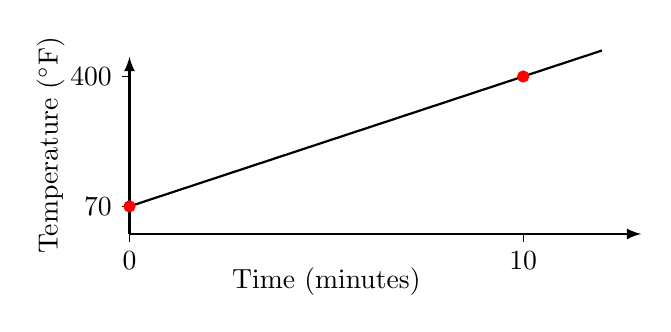
\begin{tikzpicture}[x=5mm,y=0.05mm,>=latex]
      \draw[thick,black,->] (0,0) -- (13,0);
      \draw[thick,black,->] (0,0) -- (0,450);
      \node at (5,-120) {Time (minutes)};
      \node[rotate=90] at (-2,225) {Temperature (${}^{\circ}\text{F}$)};
      \foreach \x in {0,10} 
      {
        \draw[thin,black] (\x,0) -- (\x,-1mm) node[below] {$\x$};
      }
      \foreach \y in {70,400} 
      {
        \draw[thin,black] (0,\y) -- (-1mm,\y) node[left] {$\y$};
      }
      \draw[thick,black] (0,70) -- (12,{70+33*12});
      \filldraw[red] (0,70) circle (2pt);
      \filldraw[red] (10,400) circle (2pt);
    \end{tikzpicture}
  \end{center}
  \vspace*{-0.1in}
  \pause

  \begin{enumerate}
    \setcounter{enumi}{8}
  \item  How quickly (in {\red ${}^{\circ}\text{F}/\text{min}$})\ is
    the oven heating up? 
    \begin{center}
      A$=70$
      \quad 
      B$=10$
      \quad 
      C$=40$
      \quad 
      D$=33$
      \quad 
      E$=$Other
      \qquad\pause\fbox{D}
    \end{center}
  \end{enumerate}
  \bigskip
  \pause

  Moral:  \vspace*{-0.35in}

  \begin{empheq}[box=\othermathbox]{equation*}
    \text{{\color{red}Rate of increase}}
    = 
    \text{{\color{blue}\textbf{slope}}}
  \end{empheq}
 
} 


\frame{
  \frametitle{One More Example}

  \begin{enumerate}
    \setcounter{enumi}{9}
  \item Where does the line $y=1+x$ cross the line $y=3-x$?\\
    Find both the $x$ and $y$ coordinates of the crossing point.\\
  \end{enumerate}
  \bigskip
  \pause
  
  Plan:
  \begin{enumerate}
  \item[1.]  \alert{Draw a picture!}\ showing two straight lines crossing.
  \item[2.] Solve the {\red two simultaneous equations}
  \item[3.] {\green THINK} why this gives the answer!
  \end{enumerate}
  % \vspace*{2in}
  \pause

  \begin{center}
    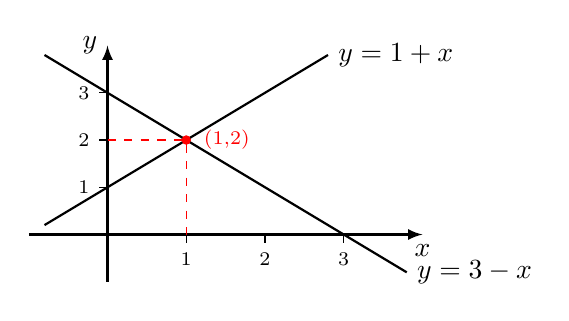
\begin{tikzpicture}[x=10mm,y=6mm,>=latex]
      \draw[thick,black,->] (-1,0) -- (4,0) node[below] {$x$};
      \draw[thick,black,->] (0,-1) -- (0,4) node[left] {$y$};
      \foreach \k in {1,2,3}
      {
        \draw[thin,black] (\k,0) -- (\k,-3pt) node[below] {$\scriptstyle\k$};
        \draw[thin,black] (0,\k) -- (-3pt,\k) node[left] {$\scriptstyle\k$};
      }
      % y=1+x:
      \draw[thick,black] (-0.8,0.2) -- (2.8,3.8) node[right] {$y=1+x$};
      % y=3-x:
      \draw[thick,black] (-0.8,3.8) -- (3.8,-0.8) node[right] {$y=3-x$};
      \draw[thin,red,dashed] (0,2) -- (1,2) -- (1,0);
      \filldraw[red] (1,2) circle (1.5pt) node[right,xshift=1mm] {$\scriptstyle(1,2)$};
    \end{tikzpicture}
  \end{center}
}


% \frame{
%   \frametitle{That's it. Thanks for being here. }

%   \begin{center}
%     
\includegraphics[scale=0.3]{Throw-It.jpg}
%   \end{center}
% }



\frame{
  \frametitle{That's it. Thanks for being here. }

  \begin{center}
    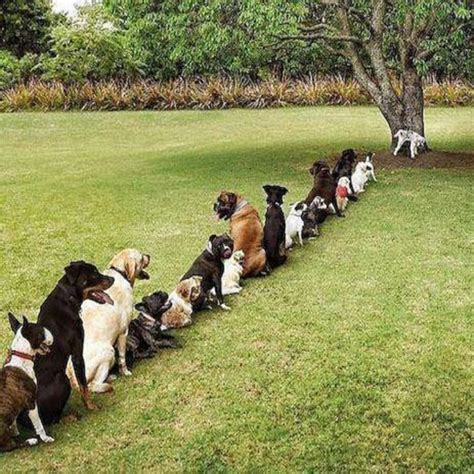
\includegraphics[scale=.4]{Lecture 4 Picture.jpg}
  \end{center}
}






\end{document}


%%% Local Variables: 
%%% mode: latex
%%% TeX-master: t
%%% End: 
